\documentclass[a4paper]{article}

\usepackage[english]{babel}
\usepackage[utf8]{inputenc}
\usepackage{amsmath}
\usepackage{graphicx}
\usepackage[colorinlistoftodos]{todonotes}
\usepackage{xcolor} % note: there's also a color package instead of xcolor
\usepackage{verbatim} % For block comments
\usepackage{tikz} % allow the drawing of images

%more complex installs with file dependancies
\usepackage[american]{circuitikzgit} % To draw digital logic circuits 
% http://texdoc.net/texmf-dist/doc/latex/circuitikz/circuitikzmanual.pdf
% circuitikz install instructions https://github.com/circuitikz/circuitikz/wiki/Installation

\label{depreciateRemove} %things that should be removed in final version but might still be useful here
\usepackage[matrix,frame,arrow]{xypic}
\usepackage{qcircuit}
%https://github.com/CQuIC/qcircuit



\label{includes} %creates a label for easy navigation

%TODO


\begin{comment}
 Add background concepts
	use balanced ternary as an intro to probability current
Physical Implementations
Brief discussion of the different architectures
Discuss access of machines themselves
Discuss how to use code API such as QiSkit
Find a way to highlight comment begins and ends
replace emphasis in biblio with italix to fix the spacing issues

\end{comment}
%%%%%%%%%%%%%%%%%%%%%%%%%%%%%%%%%%%%%%%%%%
\label{customCommands}
\definecolor{mygray}{gray}{0.6}
% Put a URL Define Here

\newcommand{\volt}[1]{${#1} V$} % shortcut to volt
\newcommand{\ohms}[1]{${#1} \Omega$} % shortcut to ohms


\begin{comment} % test circuit, not error free but draws well, fix in later revision
\begin{circuitikz}
\draw (0,0) to[R=\ohms{1}, i=?, \volt{84}] (2,0) --
(2,2) to[V=\volt{84}] (0,2)
-- (0,0);
\end{circuitikz}
\end{comment}



%%%%%%%%%%%%%%%%%%%%%%%%%%%%%%%%%%%%%%%%%%
\title{A Brief Introduction to Quantum Computing from the Perspective of Ladder Logic}

\author{Jerry Kensler}

\date{\today}

\begin{document}
\maketitle


\begin{figure}
	\centering
\begin{abstract}


While Quantum Computing is a fairly advanced topic, it suffers from a perception of complexity beyond what is reasonable for the actual subject matter.  This paper provides a means to take that perception and bring it down to a more realistic level.  The primary targets of this paper are students currently enrolled in or freshly graduated from an electrical engineering or similar program; however, any individual with a base knowledge in programming or digital logic should be able to gain some level of benefit.

Keywords:  Quantum, QISKit, Computing, Ladder, Logic, QASM, Introduction
% Need to reword this section, Find the abstract from source and merge the two
% Author note: the intention of this paper is to fill some of the skill gap many novices encounter in learning quantum computing.  By no means should this be considered an all-encompassing guide to the subject matter.
\end{abstract}
\end{figure}

\newpage %looks better as it's own page

\section{Introduction}
\label{sec:introduction}

%Explain the context of the experiment here. Why is condensed matter physics interesting or important?
%Optional things you could talk about (but don't have to -- this is up to you): transistors, computers, Quantum computers, fundamental knowledge (e.g. the resistance quantum).

%Briefly explain what methods you will use in the experiment, and what values you will extract from the data.

%For this section and all following sections: If you refer to an equation, previous result or theory that is not regarded as common knowledge, then cite the source (article or book) where you found this. For example, you can cite the Nano 3 Lecture notes \cite{nano3}.

%This section is for context.  The how, and why.  From here on out, if I refer to a theory that isn't common knowledge, cite the source. \cite{junctNew}.

Make no mistake, quantum physics as a whole is an exceptionally advanced topic.  The type of scenarios it brings to the table can be almost mind boggling at times \cite{mindBoggle}.  Add to this a slew of misleading analogies and the fact that "Qubit" may refer to any number of technologies, such as ion traps, superconducting qubits, or spin qubits and it's no wonder that people get confused.   With all of that said, while quantum computing does use the underlying principals of quantum mechanics, it is still nothing more than a programming architecture.  To put this statement in another context, an individual does not need to understand how to bias a transistor to be good at programming in C.

\subsection{Use Case for Quantum Computing} 
Quantum computing is what's called a Disruptive Emergent Technology.  Meaning, as far as industry is concerned, the implementation of these concepts have not only never been seen in any technology prior, but they also have the potential to revolutionize how things are done should these implementations prove successful.  Quantum computing is not a magic bullet that can handle every problem; however, it does have the potential to be exceptionally good at problems that current technology has issues solving.  Examples of such problems can be as varied as weather prediction, factoring \cite{shorsAlgorithm}, or even protein folding \cite{dwavepfold}. 

\subsection{Relevance to Reader} %AKA, why should you care
To avoid mincing words or dancing around the point, all that is fine, but this leads to the famous words (paraphrased ,of course) uttered at one point by nearly every person between the ages of twelve and nineteen: "Why should I care?".  To that, there are two primary categories of answers.  First, advances in technology usually creates a higher standard of living, in the case of quantum computing, these advances may end up finding the cure to debilitating ailments, reducing cost of living, or even allowing for a faster, more secure means to transport data (Quantum Internet \cite{qinternetNature}).  The second category deals with economics, the reality of the situation is that there aren't enough people who are skilled in this area to fit the demand \cite{qc5ycommercialize}.  Meaning, not only are jobs available to those with the skills to fill the required roles, but due to the shortage of supply when compared to the demand, these jobs generally pay quite well. 


\section{Background Concepts}
\label{sec:backgroundconcepts}
%brief intro to this section, needs rewording
%This section is not meant to be an exhaustive list, but, in my personal experience, learning about the background concepts below will greatly assist a person’s ability to better understand quantum computing.  The following sections will provide a brief explanation of the concepts.
In order to avoid excessive noise, this paper assumes the reader has some basic knowledge of programming as well as electronics.  It will not go into depth with much of the math, instead focusing primarily on the act of programming itself.  There are many topics which should be covered if one wishes to become skilled in quantum computing, most of which the reader will need to research on their own time; however, the sections below should provide enough context in order to provide a suitable foothold should one wish to continue with the subject.




\subsection{Removing Misleading Assumptions}
The first and easily one of the most important concepts in quantum computing is to understand that the general public and most media 'experts' do not work in the field of quantum computing.  Therefore, it is important to note that many of the common assumptions people tend to have can be misleading or plain wrong due to lack of context or the background knowledge required to properly articulate the concepts at hand.\newline
\newline
One prime example of this is Erwin Schrödinger and the concept of Schrödinger's cat.  To preface, this is not at all meant to downplay or discredit his work, merely to illustrate that without proper context even an otherwise correct statement from a Nobel laureate can be misconstrued.  \newline
\newline %helpful link to brush up https://en.wikipedia.org/wiki/Copenhagen_interpretation
To briefly summarize, Schrödinger's cat is a brilliant thought experiment meant to illustrate a potential paradox present within the Copenhagen interpretation of quantum mechanics.  This thought experiment was meant to highlight the bizarre nature of EPR (Einstein, Podolsky, Rosen), or superposition states.  This is demonstrated via a cat, radioactive particle, flask of poison, and a Geiger counter being sealed in a theoretical box.  Should the counter detect radioactivity, the flask would be broken causing the cat to die immediately.  Under the Copenhagen interpretation of quantum mechanics, this cat should be considered simultaneously both alive and dead, however, looking into the sealed box will reveal either a very scared cat, or a testament to animals killed in the name of science. \newline
\newline
 In context, this is meant to demonstrate the concepts of complex, superimposed states collapsing upon measurement. For better or worse, this concept of a not dead, yet dead cat in a box has spread like wildfire, it has become the cornerstone of what the public sees as quantum computing. This has allowed the idea that the quantum state is both 1 and 0 to become the very first thing that anyone learns in regards to quantum computing.  While this statement is not technically wrong, it is fundamentally incomplete. In many ways, it's similar to the question "which came first: the chicken, or the egg?", the answer to which can only be something along the lines of 'invalid question', as it not only fails to define what denotes the term chicken, but it also leads the individual being asked to assume the term 'egg' is specifically in the context of a chicken egg. \newline
 \newline
 In reality, a better way to think of this is through vectors and complex numbers.  The value is in fact both 1 and 0, but it's that way not because it is two things in a binary sense, but because it is a complex mixing of both.  To put this back into cat analogies, let's take the premise back to the start.  There is a cat, that cat is now infected with a zombie pathogen.  For all purposes, the cat is neither alive, nor dead, as it cannot cleanly fit into either category, yet it does have many of the defining characteristics that comprise both.  From here, the cat is injected with an antidote,  being a rushed marvel of medicine meant to save the feline race, it will near instantly result in either a complete cure or certain death for our kitten subject.  For this analogy, the zombified state represents the ability of qubits to be in a mixed state, the antidote representing the act of measuring this mixed state and thus collapsing the end result into a binary value: 1 or 0, alive or dead.


\subsection{Balanced Ternary} %The basics from the ground up
%note: blanaced ternary is not, strictly speaking a core mechanic in quantum computing.  However, it could serve as a gentle introduction to non-binary coding for many students.  A bridge between hard digital and the strangeness of qubits

Balanced Ternary is not, strictly speaking a part of quantum computing, so with that knowledge, it may seem like a strange item to include as background information when discussing the subject. However, given this author's personal experience, it is nearly ideal to serve not only as a bridge to more advanced concepts but also as a demonstration of why said concepts are important. \newline
\newline
To do this, a brief nod to what numbers are at their core is needed. It's pretty obvious to most, but numbers are nothing more or less than a way to categorize quantity.  This concept of quantity is important as it is independent of stylistic choices such as base or notation.  In programming, binary is frequently used as it reflects the power state of transistors within the register.  For most general cases, this works quite well allowing for any number of tricks, or bit-hacks, to be employed to speed things up.  However, unsigned binary does have an Achilles' heel in that due to its basis in positive numbers, there is no simple way to show when a number is negative on hardware \footnote{Note: the "-" symbol seen in both binary and standard decimal is not a representation of quantity, it's more akin to a shorthand for the operation of 0 - Quantity, and thus it's fairly difficult to represent in hardware}.  To do so, one needs to employ a tactic such as the IEEE 754 standard, adding much more complexity than would otherwise be necessary.  One way to circumvent this issue is to use a balanced number system such as balanced ternary. \newline
\newline
These systems work by designating symbols as pre-signed.  In the case of balanced ternary, the symbols are designated as "0; +; -" and they represent "$3^{(s*n)}$" with "n" being the index number starting at zero from right to left and "s" being the sign as denoted by the "+" for positive, "-" for negative, or "0" for null quantity \footnote{ This notion of sign being a property of quantity will become relevant in later sections (~\ref{ternaryRelevance}), but for now, it is acceptable to use this idea as a base case.}.  From there it is a simple matter of adding the positive and negative values up in order to get the end result (see Table~\ref{tab:ternary}, for example and comparison between bases).

\begin{table} %Table used to illustrate comparison between bases
	\centering
	\begin{tabular}{l|l|l} % Justification l-left, c-center, r-right
		Signed Decimal & Binary (IEEE 754*) & Balanced Ternary \\\hline %might remove the 754 example if it becomes an issue to clarity
		0 & 0 & 0 \\
		3 & 11 & 10 \\
		5 & 101 & + 0 - \\
		-254 & 11000011011111100000000000000000* & - 0 0 - + - \\ % -3^5 + 0 + 0 - 3^2 + 3^1 -3^0
	\end{tabular}
	\caption{\label{tab:ternary}comparison table showing equivalent numbers in different display forms}
\end{table}

\section{Advanced Concepts}
\label{sec:AdvConcepts}

%helpful link: https://arxiv.org/pdf/quant-ph/0406003.pdf Q-circuit latex tutorial
% https://www.media.mit.edu/quanta/qasm2circ/
%https://github.com/CQuIC/qcircuit Qcircuit package location
%https://tex.stackexchange.com/questions/32839/drawing-circuit-diagrams-with-logic-gates-in-latex
%self note: tons of comments here


\begin{comment} % A helpful Demo circuit graphic
\begin{circuitikz} 
	\draw
(0,2) node[and port] (myand1) {}
(0,0) node[and port] (myand2) {}
(2,1) node[xnor port] (myxnor) {}
(myand1.out) -- (myxnor.in 1)
(myand2.out) -- (myxnor.in 2);
\end{circuitikz}
\end{comment}

\subsection{Reversible Logic Gates} %The basics from the ground up
%there was a time when reversible logic was seen as a fatal flaw in QC, but some dude who was pretty clever figured out any standard logic gate could be simulated within reversible logic
A more advanced concept that is still core to quantum computing is the idea of reversible logic gates. Normally when it comes to digital logic inputs and outputs are decoupled. Consider the digital logic circuit as seen in Figure~\ref{Circuit:1}.  In this circuit, there are three inputs and a single output, even knowing the gate layout and the end value of $f_{1}$, the best that could be done for determining the input values is narrowing it to a range of possibilities as all the values have been combined into one, irreversible output. Now consider the reversible logic circuit as seen in Figure~\ref{Circuit:2}, while the notation may be unfamiliar\footnote{This notation is that of a simple quantum ladder logic circuit, the elements of which will be covered in a following section}, each input has its own unique output.  Due to this, so long as one knows what gates are in the circuit and what the output values are, the input values can be derived relatively easily.

%consider deleting circuitikz if it isn't used elsewhere


\begin{figure}
%	\centering
\label{tikzSettings} %in case it needs to move up
\usetikzlibrary{arrows, shapes.gates.logic.US, calc}
\tikzstyle{branch}=[fill, shape=circle, minimum size=3pt, inner sep=0pt]
\begin{tikzpicture}
\node (x) at (0, 2) {$x_{1}$};
\node (y) at (0, 1) {$x_{2}$};
\node (z) at (0, 0) {$x_{3}$};

\node[not gate US, draw] at ($(x) + (0.8, 0)$) (notx) {};
\node[not gate US, draw] at ($(y) + (0.8, 0)$) (noty) {};
%\node[and gate US, draw, rotate=0, logic gate inputs=nnnn] at ($(noty) + (2, 0.085)$) (xory) {};
\node[or gate US, draw, rotate=0, logic gate inputs=nnn] at ($(noty) + (2, 0.085)$) (xory) {};

\draw (x) -- (notx.input);
\draw (y) -- (noty.input);

\path ($(notx.input) + (0.2, 0)$) -- coordinate (puntx) (x |- notx);
%\draw (x) -- (puntx) node[branch] {} |- ($(notx.output) + (0.4, 0.4)$) |- (xory.input 1);

\draw (notx.output) -- ([xshift=0.2cm]notx.output) |- (xory.input 1);
\draw (noty.output) -- ([xshift=0.2cm]noty.output) |- (xory.input 2);
\draw (z) -| ($(noty.output) + (0.2, -0.5)$) |- (xory.input 3);

\draw (xory.output) -- node[above]{$f_{1}= \bar x_{1} + \bar x_{2} + x_{3}$} ($(xory) + (3.5, 0)$);
%\draw (xory.output) -- node[above]{$\overline{x + \bar x + \bar y + z}$} ($(xory) + (3, 0)$);
\end{tikzpicture}
\caption{Digital Logic Circuit}\label{Circuit:1}
\end{figure}

%\begin{comment}%debugging

\begin{figure}
 %helpful for understanding the syntax https://github.com/CQuIC/qcircuit/blob/master/Qtutorial.tex


%\small \begin{verbatim} %verbatim displays the code itself instead of rendering it
\[\Qcircuit @C=1em @R=0.5em @!R { %rows and columns, pretty standard
	 \lstick{\psi} & \targ & \targ & \qw & \targ & \meter \\
	 \lstick{\psi} & \ctrl{-1} & \qw &\qw & \qw & \meter \\
	 \lstick{\psi} & \qw & \ctrl{-2} & \qw & \qw & \meter \\
	 \lstick{\psi} & \qw & \qw & \qw & \ctrl{-3} & \meter\\
}\]
%\end{verbatim}}
%&\lstick{\ket{\psi}}
	\caption{Reversible Logic Circuit}\label{Circuit:2}
\end{figure}

%\end{comment}%debugging


\subsection{Probability Amplitudes}
\label{ternaryRelevance} %allows linking to this spot regardless of location
\label{currentSpot}

\section{Quantum Ladder Logic}




\section{Experiment 1-2 pages}
\begin{comment} %comment out defaults
\subsection{Fabrication}
Explain a step-by-step recipe for fabrication here. How long did you etch and why? What is an Ohmic contact?
\subsection{Experimental set-up}
Explain the experimental set-up here.

\end{comment} %comment out defaults

\section{Results and interpretation 2-3 pages}
Show a graph of the longitudinal resistivity ($\rho_{xx}$) and Hall resistivity ($\rho_{xy}$) versus magnetic field, extracted from the raw data shown in figure \ref{fig:data}. You will have the link to the data in your absalon messages, if not e-mail Guen (guen@nbi.dk). Explain how you calculated these values, and refer to the theory.

%\begin{figure}
%\centering
%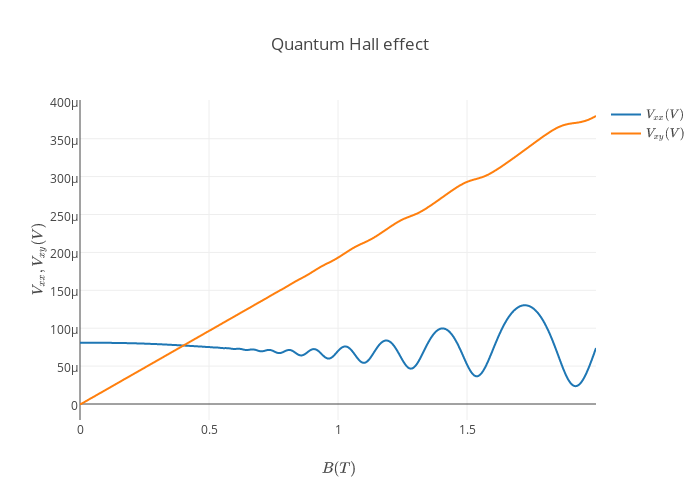
\includegraphics[width=1\textwidth]{raw_data.png}
%\caption{\label{fig:data}Raw (unprocessed) data. Replace this %figure %with the one you've made, that shows the resistivity.}
%\end{figure}
\begin{comment} %comment out defaults
\subsection{Classical regime}
Calculate the sheet electron density $n_{s}$ and electron mobility $\mu$ from the data in the low-field regime, and refer to the theory in section \ref{sec:theory}. Explain how you retrieved the values from the data (did you use a linear fit?).
Round values off to 1 or 2 significant digits: 8.1643 ~= 8.2. Also, 5e-6 is easier to read than 0.000005.

!OBS: This part is optional (only if you have time left).
Calculate the uncertainty as follows: \newline $u(f(x, y, z)) = \sqrt{(\frac{\delta f}{\delta{x}} u(x))^{2} + (\frac{\delta f}{\delta{y}} u(y))^{2} + (\frac{\delta f}{\delta{z}} u(z))^{2}}$, where $f$ is the calculated value ($n_{s}$ or $\mu$), $x, y, z$ are the variables taken from the measurement and $u(x)$ is the uncertainty in x (and so on).

\subsection{Quantum regime}
Calculate $n_{s}$ for the high-field regime.
Show a graph of the longitudinal conductivity ($\rho_{xx}$) and Hall conductivity($\rho_{xy}$) \textbf{in units of the resistance quantum} ($\frac{h}{e^{2}}$), depicting the integer filling factors for each plateau.
Show a graph of the plateau number versus its corresponding value of $1/B$. From this you can determine the slope, which you use to calculate the electron density.
Again, calculate the uncertainty for your obtained values.
\end{comment} %comment out defaults

\section{Discussion 1/2-1 page}
Discuss your results. Compare the two values of $n_{s}$ that you've found in the previous section. Compare your results with literature and comment on the difference. If you didn't know the value of the resistance quantum, would you be able to deduce it from your measurements? If yes/no, why?

\begin{comment} %comment out defaults

\newpage
\section{Some LaTeX tips}
\label{sec:latex}
\subsection{How to Include Figures}

First you have to upload the image file (JPEG, PNG or PDF) from your computer to writeLaTeX using the upload link the project menu. Then use the includegraphics command to include it in your document. Use the figure environment and the caption command to add a number and a caption to your figure. See the code for Figure \ref{fig:frog} in this section for an example.

%\begin{figure}
%\centering
%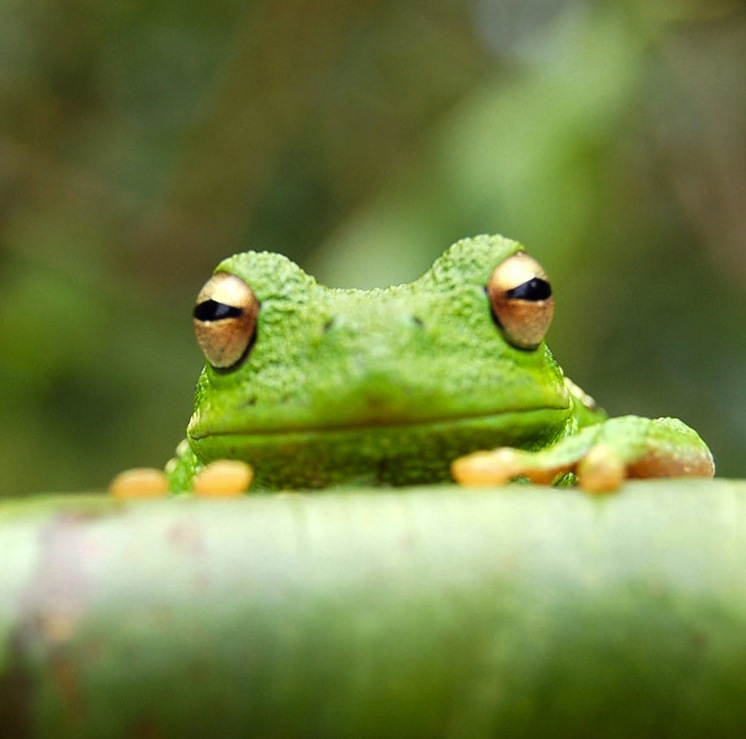
\includegraphics[width=0.3\textwidth]{frog.jpg}
%\caption{\label{fig:frog}This frog was uploaded to writeLaTeX via %the project menu.}
%\end{figure}



\subsection{How to Write Mathematics}

\LaTeX{} is great at typesetting mathematics. Let $X_1, X_2, \ldots, X_n$ be a sequence of independent and identically distributed random variables with $\text{E}[X_i] = \mu$ and $\text{Var}[X_i] = \sigma^2 < \infty$, and let

\begin{equation}
S_n = \frac{X_1 + X_2 + \cdots + X_n}{n}
      = \frac{1}{n}\sum_{i}^{n} X_i
\label{eq:sn}
\end{equation}

denote their mean. Then as $n$ approaches infinity, the random variables $\sqrt{n}(S_n - \mu)$ converge in distribution to a normal $\mathcal{N}(0, \sigma^2)$.

The equation \ref{eq:sn} is very nice.

\subsection{How to Make Sections and Subsections}

Use section and subsection commands to organize your document. \LaTeX{} handles all the formatting and numbering automatically. Use ref and label commands for cross-references.

\subsection{How to Make Lists}

You can make lists with automatic numbering \dots

\begin{enumerate}
\item Like this,
\item and like this.
\end{enumerate}
\dots or bullet points \dots
\begin{itemize}
\item Like this,
\item and like this.
\end{itemize}
\dots or with words and descriptions \dots
\begin{description}
\item[Word] Definition
\item[Concept] Explanation
\item[Idea] Text
\end{description}



We hope you find write\LaTeX\ useful, and please let us know if you have any feedback using the help menu above.


\end{comment} %comment out defaults


%%%%%%%%%%%%%%%%%%%%%%%%%%%%%%%%%%%%%%%%%%%%%%%%%%%%%%%%%%%%%%%%%%

\begin{thebibliography}{9}
	\label{sec:bibliography} %allows for quick navigation via side bar	
%========================================================================================

%\bibitem{template}
%	AuthorLast, AuthorF MI. \emph{"TitleOfSource.} OptionalCityOfPublication, OptionalDateOfOriginalPublication" TitleOfContainer. Version, OtherContributers, NumberSuchAsEpisodeVolume. Publisher, PublicationDate, LocationSuchAsPageNumberOrURL_Or_DOI. AccessedDayMonthSpelledOutYear

%https://owl.english.purdue.edu/owl/resource/747/01/

%========================================================================================
\bibitem{qcircuitLatex}
	University of New Mexico. \emph{"Q-circuit Tutorial"} ARXIV, August 24 2004, eprint arXiv:quant-ph/0406003. Bryan Eastin, Steven T. Flammia, Department of Physics and Astronomy. Accessed May 20 2018. https://arxiv.org/pdf/quant-ph/0406003.pdf 

\bibitem{qc5ycommercialize}
	Google Quantum AI Laboratory. \emph{"Commercialize quantum technologies in five years"}. March 03 2017. Masoud Mohseni, Peter Read, Hartmut Neven, Sergio Boxio, Vasil Denchev, Ryan Babbush, Austin Fowler, Vadim Smelyanskiy, John Martinis.  Accessed May 06 2018.  https://www.nature.com/news/commercialize-quantum-technologies-in-five-years-1.21583

\bibitem{qinternetNature}
	Castelvecchi, Davide. \emph{"The quantum internet has arrived (and it hasn’t)"}.  February 14 2018, Nature.  Accessed February 20 2018. https://www.nature.com/articles/d41586-018-01835-3

\bibitem{shorIllDoIt}
	Aaronson, Scott. \emph{"Shor, I'll do it"}. February 24 2007, Shtetl-Optimized. Accessed December 02 2016. https://www.scottaaronson.com/blog/?p=208

\bibitem{shorsAlgorithm}
	Shor, Peter W. \emph{"Polynomial-Time Algorithms for Prime Factorization and Discrete Logarithms on a Quantum Computer"}. ARXIV, August 30 1995, eprint arXiv:quant-ph/9508027. Accessed August 30 2017. https://arxiv.org/abs/quant-ph/9508027   

\bibitem{laymanShor}
	Forum Users. \emph{"Prime Numbers: In Layman's Terms, How does Shors Algorithm Work?"}, October 9 2012. Cryptography Stack Exchange.  StackExchange, Accessed March 4 2017. https://crypto.stackexchange.com/questions/3932/in-laymans-terms-how-does-shors-algorithm-work

\bibitem{junctNew}  
	Richard Newrock,
	\emph{"What are Joesphson Junctions? How do they work?"}
	Scientific American
	
\bibitem{mindBoggle}
	Moskowitz, Clara. \emph{"New Particle Is Both Matter and Antimatter"}. October 2 2014, Scientific American. Accessed April 4 2018. https://www.scientificamerican.com/article/majorana-particle-matter-and-antimatter/

\bibitem{dwavepfold}
	Brumfiel, Geoffrey. \emph{"D-Wave quantum computer solves protein folding problem"}. August 17 2012. Nature. Accessed August 1 2017. http://blogs.nature.com/news/2012/08/d-wave-quantum-computer-solves-protein-folding-problem.html
	

\bibitem{mitqcshor}
	Shor, Peter. \emph{"Quantum Computation".} MIT OpenCourseware. Massachusetts Institute of Technology, 2003,18.435J / 2.111J / ESD.79J, \newline https://ocw.mit.edu/courses/mathematics/18-435j-quantum-computation-fall-2003/

\bibitem{cmuqc15}
	O'Donnell, Ryan. Wright, John. \emph{"Quantum Computation and Information".} Carnegie Mellon University, 2015, 15-859BB, \newline https://www.cs.cmu.edu/~odonnell/quantum15/

\bibitem{qazoo}
	Jordan, Stephan. \emph{"Quantum Algorithm Zoo".} National Institute of Standards and Technology (NIST),  https://math.nist.gov/quantum/zoo/
	
\bibitem{qiskit}
	QISKit. \emph{"QISKit."} https://github.com/QISKit. Accessed: February 14 2018
\begin{comment} % More info on QISKit
https://github.com/QISKit
  https://github.com/QISKit/ibmqx-user-guides
  https://github.com/QISKit/qiskit-tutorial
     https://github.com/QISKit/qiskit-tutorial/blob/master/INSTALL.md
        https://datascience.ibm.com/
        https://medium.com/qiskitters/qiskit-turns-one-looking-back-cbc2c48d7a95
     https://github.com/QISKit/qiskit-tutorial/blob/master/hello_world/quantum_emoticon.ipynb
\end{comment} % End QISKit extra info

\bibitem{qbenchgame}
	Wooten, James. \emph{"Using a Simple Puzzle Game to Benchmark Quantum Computers".} Medium, January 16 2018. https://medium.com/@decodoku/understanding-quantum-computers-through-a-simple-puzzle-game-a290dde89fb2

\begin{comment}% Further info on the benchmark game

https://mybinder.org/v2/gh/decodoku/A_Game_to_Benchmark_Quantum_Computers/master?filepath=Play_Quantum_Awesomeness.ipynb
    Also seen below, using a python game to illustrate quantum noise

https://medium.com/@decodoku/quantum-computation-in-84-short-lines-d9c7c74be0d0
    https://medium.com/@decodoku
        https://mybinder.org/v2/gh/decodoku/A_Game_to_Benchmark_Quantum_Computers/master?filepath=Play_Quantum_Awesomeness.ipynb
            Also seen above
\end{comment}% End further info on quantum benchmark game

\bibitem{algoassert} %finish this up
	Gidney, Craig. \emph{"Algorithmic Assertions"} Google AI, http://algassert.com/. Accessed: \date{\today}
\begin{comment} % helpful links on the site
http://algassert.com/quantum/2014/03/07/Building-your-own-Quantum-Fourier-Transform.html
	http://algassert.com/post/1704
		circuit width talk
	http://algassert.com/post/1628
		swapping to teleporting with simple circuit moves
	http://algassert.com/post/1618
		Affecting atoms by looking at emitted light
	http://algassert.com/quantum/2015/05/01/Quantum-Network-Flow-Puzzle.html
\end{comment} % End helpful links on the site


%========================================================================================

%\bibitem{template}
%	AuthorLast, AuthorF MI. \emph{"TitleOfSource.} OptionalCityOfPublication, OptionalDateOfOriginalPublication" TitleOfContainer. Version, OtherContributers, NumberSuchAsEpisodeVolume. Publisher, PublicationDate, LocationSuchAsPageNumberOrURL_Or_DOI. AccessedDayMonthSpelledOutYear

%https://owl.english.purdue.edu/owl/resource/747/01/

%========================================================================================

\begin{comment} %Start block comment


========Old Section=====

Gates: http://www.inetdaemon.com/img/gates.gif

https://inspirehep.net/record/1320783/files/fig1b.png


========================
===========Things Used=============

https://people.eecs.berkeley.edu/~vazirani/quantum.html



https://console.bluemix.net/dashboard/apps/
  This is Watson and other things


https://github.com/github/gitignore/blob/master/TeX.gitignore
  This is the gitignore settings nessisary to not constantly upload aux files when using LaTeX

http://web.mit.edu/rsi/www/pdfs/new-latex.pdf
  How to write in LaTeX

https://quantumexperience.ng.bluemix.net/qx/tutorial?sectionId=full-user-guide&page=introduction
	IBM Quantum Experience User guide
	https://quantumexperience.ng.bluemix.net/qx/community/question?questionId=e4b7b71ae47096a45e70fbcde8aee687
		A grover's algorithm implementation


http://paulklemm.com/blog/2014-07-16-use-github-for-scientific-writing/

https://arxiv.org/abs/1804.03719
	Quantum Algorithm Implementations for Beginners


https://quantumcomputing.stackexchange.com/
    --A place where people can ask questions and get help with quantum computing
    https://quantumcomputing.stackexchange.com/questions/1404/will-deep-learning-neural-networks-run-on-quantum-computers
	Will Neural Networks run on Quantum Computers

https://www.quantiki.org/wiki/basic-concepts-quantum-computation

https://www.media.mit.edu/quanta/qasm2circ/
	to draw circuits
https://tex.stackexchange.com/questions/9767/whats-a-good-package-for-typesetting-quantum-circuits

http://kim.oyhus.no/QuantumMechanicsForProgrammers.html


https://arxiv.org/pdf/1610.06980.pdf
	A paper on IBM Q that needs translation but looks relevant

https://arxiv.org/pdf/quant-ph/0308074.pdf
	Probability amplitute in Quantum-Like Games

https://arxiv.org/abs/1205.4926
	Quantum Delayed Choice Experiment


https://www.quora.com/Is-it-possible-to-build-a-very-primitive-quantum-computer-at-home


https://arxiv.org/pdf/quant-ph/0503228v1.pdf
	The Physics of Factorization

https://arxiv.org/abs/1505.04577
	Analogue algorithm for parallell factorization of an exponential number of Large integers 1. Theoretical Description

http://stationq.github.io/Liquid/
	Language integrated Quantum Op Simulator
		Don't remember using, but it was with the links so I'll check on it later

https://kukuruku.co/post/quantum-circuits-methods-and-techniques/

https://hackaday.com/2017/01/24/the-birth-of-quantum-electrodynamics/

https://www.media.mit.edu/quanta/qasm2circ/

https://www.dwavesys.com/software



==========Stuff that is handy to have=============

http://backreaction.blogspot.com/2017/08/the-annotated-math-of-almost-everything.html?spref=tw

https://hackaday.com/2018/01/24/quantum-weirdness-in-your-browser/

Github Tutorial: 
  https://try.github.io/

https://www.overleaf.com/latex/templates/
  LaTeX Document templates for things like Resumes and Academic Reports

https://hackaday.com/2018/04/19/when-4-1-equals-8-an-advanced-take-on-pointers-in-c/
  A good tutorial on pointers in C



========================
==========Might use section==============
https://www.overleaf.com/latex/examples/title-page-with-logo/hrskypjpkrpd

https://github.com/adamisntdead/QuSimPy
  A quantum simulator someone wrote in python,  Could be useful to reference and see how they did things

Microsoft Q#
	https://docs.microsoft.com/en-us/quantum/?view=qsharp-preview
	https://docs.microsoft.com/en-us/quantum/quantum-writeaquantumprogram?view=qsharp-preview&tabs=tabid-vs2017
%
%============
%=========Extended Reading?================

%
%Data structure search visualization
%	https://visualgo.net/en
%
%
%https://www.nextplatform.com/2017/03/29/neuromorphic-quantum-supercomputing-mesh-deep-learning/
%
%https://arstechnica.com/science/2017/04/the-route-to-high-speed-quantum-computing-is-paved-with-error/
%
%https://drstienecker.com/tech-332/5-ladder-logic/
%
%https://www.youtube.com/user/LookingGlassUniverse/videos
%	videos on quantum computing and weirdness
%
%https://journals.aps.org/prl/abstract/10.1103/PhysRevLett.69.2881
%
%https://arxiv.org/abs/quant-ph/0006004
%	Fast paralell Circuits for the Quantum Fourier Transform
%
%https://www.nature.com/news/quantum-computers-ready-to-leap-out-of-the-lab-in-2017-1.21239
%
%https://www.youtube.com/watch?v=N6w9Pq6Q9OM
%	Spintronics Explanation
%
%=========Misc Helpful Links ===============
%
%news.ycombinator.com
%	Tech news
%
%hackaday.com
%	Various projects


  
%%%%EXAMPLE MLA FORMAT

%https://owl.english.purdue.edu/owl/resource/747/12/
%


%https://owl.english.purdue.edu/owl/resource/747/01/



\end{comment}
\end{thebibliography}
\begin{scriptsize}
\textcolor{mygray}{For extended reading list, consult source code, available at: \newline https://www.github.com/Macrofarad/ABriefIntroductionToQuantumComputingFromThePerspectiveOfLadderLogic}

%Edit as url changes, suggest placing completed project as new repository with a slightly better name
\end{scriptsize} %size list: Huge, huge, LARGE, Large, large, normalsize, small, footnotesize, scriptsize, tiny
\end{document}
